%! TeX program = xelatex
\documentclass{standalone}
\input{../tikz.tex.preamble}

\begin{document}
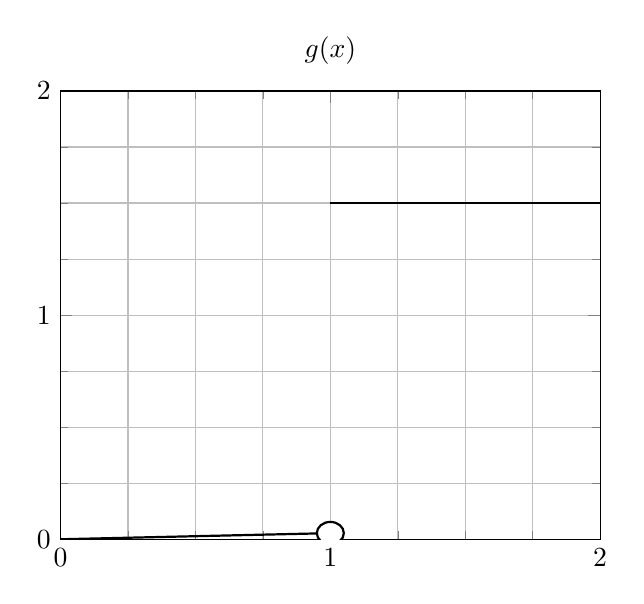
\begin{tikzpicture}
  \begin{axis}[
    xmin=0, xmax=2, ymin=0, ymax=2, 
    xtick={0, 1, 2},
    ytick={0, 1, 2},
    grid=both, minor tick num=3,
    title={\(g(x)\)},
    ]
    \addplot[thick, domain=0:1] {sin(x*(pi/2))} node (A) {};
    \addplot[thick, domain=1:2] {1.5};

    \draw[fill=white, thick] (A) circle (0.05);
  \end{axis}
\end{tikzpicture}
\end{document}
